\maketitle{}
\section{ State Management - @ngrx/store }

Ngrx/store is a layer on top of Redux. It is a state management tool that was
originally created, in order to solve two way binding performance issues within
Angular. \footnote{Need to further bring source for this one}. It then extended
as a way to bring redux natively to Angular, with the use of Observables.

Let's dive into integrating @ngrx/store into our app. \marginpar{This particular
component has been written in the fashion of TDD. However, another chapter
will be dedicated to TDD/BDD in order to specify this point specifically.}

\subsection{ Using nx ngrx to Generate State }

\subsubsection{ Create root state using nx ngrx }

First we are going to generate an empty root, for our StoreModule, as well as
our EffectsModule. Our StoreModule is responsible as a singular store object,
which will be holding all of store data. Our EffectsModule is a singular effects
object, which will be holding all of our effects. \footnote{We will discuss
effects in more detail later}

\begin{lstlisting}[language=Bash]
ng generate ngrx app --module=apps/angular-pixel-illustrator/src/app/app.module.ts --onlyEmptyRoot
\end{lstlisting}

\subsubsection{ Create component state using nx ngrx }

Next, we are going to create state for our choose-size component. This is done
with ease using nx ngrx \footnote{Trust me, I've been in situations where I
was not using a CLI. It is not good news}

Run the following command:
\begin{lstlisting}[language=Bash]
ng generate ngrx choose-size --module=apps/angular-pixel-illustrator/src/app/components/choose-size/choose-size.module.ts
\end{lstlisting}

This will generate the following files:
\begin{lstlisting}[language=Bash]
create apps/angular-pixel-illustrator/src/app/components/choose-size/+state/choose-size.actions.ts (684 bytes)
create apps/angular-pixel-illustrator/src/app/components/choose-size/+state/choose-size.reducer.ts (869 bytes)
create apps/angular-pixel-illustrator/src/app/components/choose-size/+state/choose-size.effects.ts (859 bytes)
create apps/angular-pixel-illustrator/src/app/components/choose-size/+state/choose-size.effects.spec.ts (1070 bytes)
create apps/angular-pixel-illustrator/src/app/components/choose-size/+state/choose-size.reducer.spec.ts (364 bytes)
\end{lstlisting}
And update the choose-size module,
\begin{lstlisting}[language=Bash]
update apps/angular-pixel-illustrator/src/app/components/choose-size/choose-size.module.ts
\end{lstlisting}

\subsubsection{ High level overview of nx ngrx }
So, you might be wondering, what do those files that nx ngrx generated actually
do? It will generate three files:
\begin{enumerate}
  \item Action
  \item Reducer
  \item Effect
\end{enumerate}

In addition, nx will add Typescript enums for the action types. It will also
add a respective spec file(unit testing) for the action + reducer file.

\colorbox{darkgray}{\color{white}{Unit testing Actions?}}

Unit testing an action, would simply say, when an action is dispatched, expect
it to be of a certain type. However, enums, as well as type checking, fulfills
that obligation. Therefore, if one is using Typescript along with enums, there
should be no reason for writing unit tests.

\subsubsection{ Installing Redux Dev Tools }
A state environment is incomplete without proper devtools. In particular, being
able to see an action fired, as well as the complete state of any given time,
is invaluable.

Google, "redux Devtools"\footnote{In a book format, in my humble opinion, more
valuable than a link}. It is offered by remotedev.io.

With the chooseSize ngrx nx command, we just made, you should see something like
this:

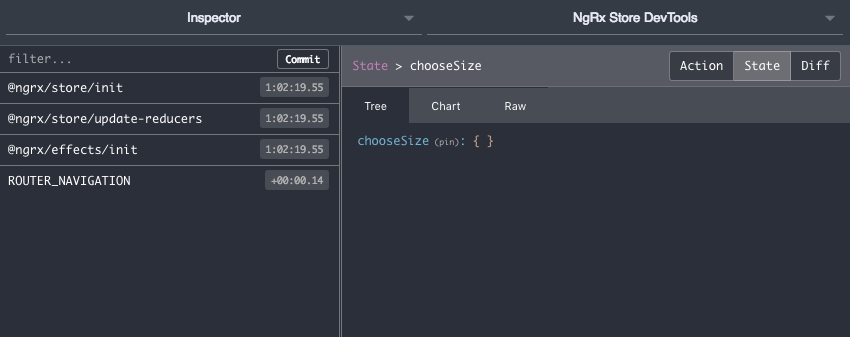
\includegraphics[width=13cm, height=9cm]{ngrx-store/redux-store}
